\documentclass[11pt,]{article}
\usepackage{lmodern}
\usepackage{amssymb,amsmath}
\usepackage{ifxetex,ifluatex}
\usepackage{fixltx2e} % provides \textsubscript
\ifnum 0\ifxetex 1\fi\ifluatex 1\fi=0 % if pdftex
  \usepackage[T1]{fontenc}
  \usepackage[utf8]{inputenc}
\else % if luatex or xelatex
  \ifxetex
    \usepackage{mathspec}
  \else
    \usepackage{fontspec}
  \fi
  \defaultfontfeatures{Ligatures=TeX,Scale=MatchLowercase}
\fi
% use upquote if available, for straight quotes in verbatim environments
\IfFileExists{upquote.sty}{\usepackage{upquote}}{}
% use microtype if available
\IfFileExists{microtype.sty}{%
\usepackage{microtype}
\UseMicrotypeSet[protrusion]{basicmath} % disable protrusion for tt fonts
}{}
\usepackage[margin=1in]{geometry}
\usepackage{hyperref}
\hypersetup{unicode=true,
            pdftitle={A User-Friendly U.S. Census Browser for R},
            pdfauthor={Kiegan Rice},
            pdfborder={0 0 0},
            breaklinks=true}
\urlstyle{same}  % don't use monospace font for urls
\usepackage{color}
\usepackage{fancyvrb}
\newcommand{\VerbBar}{|}
\newcommand{\VERB}{\Verb[commandchars=\\\{\}]}
\DefineVerbatimEnvironment{Highlighting}{Verbatim}{commandchars=\\\{\}}
% Add ',fontsize=\small' for more characters per line
\usepackage{framed}
\definecolor{shadecolor}{RGB}{248,248,248}
\newenvironment{Shaded}{\begin{snugshade}}{\end{snugshade}}
\newcommand{\KeywordTok}[1]{\textcolor[rgb]{0.13,0.29,0.53}{\textbf{{#1}}}}
\newcommand{\DataTypeTok}[1]{\textcolor[rgb]{0.13,0.29,0.53}{{#1}}}
\newcommand{\DecValTok}[1]{\textcolor[rgb]{0.00,0.00,0.81}{{#1}}}
\newcommand{\BaseNTok}[1]{\textcolor[rgb]{0.00,0.00,0.81}{{#1}}}
\newcommand{\FloatTok}[1]{\textcolor[rgb]{0.00,0.00,0.81}{{#1}}}
\newcommand{\ConstantTok}[1]{\textcolor[rgb]{0.00,0.00,0.00}{{#1}}}
\newcommand{\CharTok}[1]{\textcolor[rgb]{0.31,0.60,0.02}{{#1}}}
\newcommand{\SpecialCharTok}[1]{\textcolor[rgb]{0.00,0.00,0.00}{{#1}}}
\newcommand{\StringTok}[1]{\textcolor[rgb]{0.31,0.60,0.02}{{#1}}}
\newcommand{\VerbatimStringTok}[1]{\textcolor[rgb]{0.31,0.60,0.02}{{#1}}}
\newcommand{\SpecialStringTok}[1]{\textcolor[rgb]{0.31,0.60,0.02}{{#1}}}
\newcommand{\ImportTok}[1]{{#1}}
\newcommand{\CommentTok}[1]{\textcolor[rgb]{0.56,0.35,0.01}{\textit{{#1}}}}
\newcommand{\DocumentationTok}[1]{\textcolor[rgb]{0.56,0.35,0.01}{\textbf{\textit{{#1}}}}}
\newcommand{\AnnotationTok}[1]{\textcolor[rgb]{0.56,0.35,0.01}{\textbf{\textit{{#1}}}}}
\newcommand{\CommentVarTok}[1]{\textcolor[rgb]{0.56,0.35,0.01}{\textbf{\textit{{#1}}}}}
\newcommand{\OtherTok}[1]{\textcolor[rgb]{0.56,0.35,0.01}{{#1}}}
\newcommand{\FunctionTok}[1]{\textcolor[rgb]{0.00,0.00,0.00}{{#1}}}
\newcommand{\VariableTok}[1]{\textcolor[rgb]{0.00,0.00,0.00}{{#1}}}
\newcommand{\ControlFlowTok}[1]{\textcolor[rgb]{0.13,0.29,0.53}{\textbf{{#1}}}}
\newcommand{\OperatorTok}[1]{\textcolor[rgb]{0.81,0.36,0.00}{\textbf{{#1}}}}
\newcommand{\BuiltInTok}[1]{{#1}}
\newcommand{\ExtensionTok}[1]{{#1}}
\newcommand{\PreprocessorTok}[1]{\textcolor[rgb]{0.56,0.35,0.01}{\textit{{#1}}}}
\newcommand{\AttributeTok}[1]{\textcolor[rgb]{0.77,0.63,0.00}{{#1}}}
\newcommand{\RegionMarkerTok}[1]{{#1}}
\newcommand{\InformationTok}[1]{\textcolor[rgb]{0.56,0.35,0.01}{\textbf{\textit{{#1}}}}}
\newcommand{\WarningTok}[1]{\textcolor[rgb]{0.56,0.35,0.01}{\textbf{\textit{{#1}}}}}
\newcommand{\AlertTok}[1]{\textcolor[rgb]{0.94,0.16,0.16}{{#1}}}
\newcommand{\ErrorTok}[1]{\textcolor[rgb]{0.64,0.00,0.00}{\textbf{{#1}}}}
\newcommand{\NormalTok}[1]{{#1}}
\usepackage{graphicx,grffile}
\makeatletter
\def\maxwidth{\ifdim\Gin@nat@width>\linewidth\linewidth\else\Gin@nat@width\fi}
\def\maxheight{\ifdim\Gin@nat@height>\textheight\textheight\else\Gin@nat@height\fi}
\makeatother
% Scale images if necessary, so that they will not overflow the page
% margins by default, and it is still possible to overwrite the defaults
% using explicit options in \includegraphics[width, height, ...]{}
\setkeys{Gin}{width=\maxwidth,height=\maxheight,keepaspectratio}
\IfFileExists{parskip.sty}{%
\usepackage{parskip}
}{% else
\setlength{\parindent}{0pt}
\setlength{\parskip}{6pt plus 2pt minus 1pt}
}
\setlength{\emergencystretch}{3em}  % prevent overfull lines
\providecommand{\tightlist}{%
  \setlength{\itemsep}{0pt}\setlength{\parskip}{0pt}}
\setcounter{secnumdepth}{5}
% Redefines (sub)paragraphs to behave more like sections
\ifx\paragraph\undefined\else
\let\oldparagraph\paragraph
\renewcommand{\paragraph}[1]{\oldparagraph{#1}\mbox{}}
\fi
\ifx\subparagraph\undefined\else
\let\oldsubparagraph\subparagraph
\renewcommand{\subparagraph}[1]{\oldsubparagraph{#1}\mbox{}}
\fi

%%% Use protect on footnotes to avoid problems with footnotes in titles
\let\rmarkdownfootnote\footnote%
\def\footnote{\protect\rmarkdownfootnote}

%%% Change title format to be more compact
\usepackage{titling}

% Create subtitle command for use in maketitle
\newcommand{\subtitle}[1]{
  \posttitle{
    \begin{center}\large#1\end{center}
    }
}

\setlength{\droptitle}{-2em}
  \title{A User-Friendly U.S. Census Browser for R}
  \pretitle{\vspace{\droptitle}\centering\huge}
  \posttitle{\par}
  \author{Kiegan Rice}
  \preauthor{\centering\large\emph}
  \postauthor{\par}
  \date{}
  \predate{}\postdate{}

\usepackage{float}

\begin{document}
\maketitle

\section{Introduction}

Census data provide an important snapshot of information about a country
at different times throughout its history, and their value is difficult
to overstate. While history books present a narrative of the events that
occured, students themselves often don't get to interact with the raw
data in that learning environment. Clean and accessible census data
allow the exploration of different demographic groups over time, or
investigations of a particular period of time and what the demographic
and economic landscape looked like in the past. Even today, data about
the world around us opens a pathway for learning more about places we
haven't been and groups of people with whom we may not usually engage.

From an early point in the United States' history, there were many
``eminent men of science'' who recognized the value of the census data
and worked to aggregate and present those data. Francis A. Walker's
``Statistical Atlas of the United States'', based on the 1870 census,
was an impressive effort in aggregating population data to present them
in a visually appealing way (Office and Walker 1874). Although the
Census Bureau's ``Statistical Atlases'' eventually stopped being
created, they were an important start to the effort of visually
presenting census data to a wider public (see Figure 1).

\begin{figure}[htbp]
\centering
\includegraphics[width=0.90000\textwidth]{./figures/colored-population-stat-atlas.png}
\caption{An example of a visualization of data from the Statistical
Atlas based on the 1870 census.}
\end{figure}

Today, as methods of data analysis and visualization continue to be
developed and improved, access to census data allows us to look back on
that history and explore, synthesize, and visualize the information.
When aggregated and presented in a clear manner, viewers can learn more
about patterns in many different parts of the population. A 2007 paper
about the Statistical Atlas discusses just how much information is
present in those original charts and demonstrates several other ways of
presenting the information that can be found therein (Hofmann 2007).

Ever-improving visualization and data-wrangling methods in R (R Core
Team 2015) give those interested in statistical graphics a wealth of
opportunities to explore and learn from data; in particular,
incorporating user interactivity using Shiny has revolutionized the way
statisticians share and communicate information (Chang et al. 2017).
However, it is difficult to make use of these tools with census data if
those data are not available and easy to explore in one location.

An inherent problem in census data is that a country's census changes
over time; the variables collected, how they are collected, and even the
locations on which they are collected are updated as the country is
formed, and subsequently grows and changes. The United States census
data are no exception to this rule. In little under two and a half
centuries, the census has taken many different forms. Data on
occupations have transformed as the employment landscape has changed;
new states have been formed, the most recent being within the last 100
years; definitions of various demographic groups and the terminology
used to describe them have been updated as the demographic makeup of the
country has changed. Each decennial census brings a different set of
variables to the table. Sometimes these variables are new things the
Census Bureau is interested in learning about, while sometimes they
remove variables that are no longer relevant or whose information is
captured elsewhere.

Unfortunately, because the founders of the U.S. Census were unable to
see 200 years into the future, those interested in working with census
data are left with quite the inescapable mess. If you want to focus in
on a particular demographic group and their journey as part of the
population of the United States, you may have ten or more different
variable names to describe that one group over the course of the census
from 1790 to 1960 - and that is just for a single group! Of course, we
cannot just simply change variable names to match our own research
needs. It is important to keep the data in their true form and be
respectful of the way in which the population was defined at different
times throughout history, even if our instinct may be to `clean' the
data by changing variable names.

This, of course, leaves the user with a wide variety of variables that
are far from consistent across years. In order to track one demographic
group across years - let alone many groups - a clean user interface that
helps users see exactly what information is available to them is a
necessity. To streamline the process and assist researchers in finding
out to what information they have access and what information they lack,
a U.S. Census Browser for R is presented as an R package, with the user
interface being a Shiny application, and the downloadable files being
`tidy' comma-separated values (csv) files that those with a minimal
amount of R experience can still process.

\section{Data Access}

There are two main datasets that contain the aggregated counts of
historical, demographic, economic, and social characteristics from the
United States decennial census. They were both collected and developed
by the Inter-University Consortium for Political and Social Research
(ICPSR). The ICPSR 3, gathered from computer-readable data collections
from the U.S. Census Bureau as well as other reports (both published and
unpublished), contains data from 1790 to 1960. The ICPSR 2896 includes
much of the same information as the ICPSR 3, and in addition also
includes a wider array of variables such as manufacturing and more
county and city-level information. The ICPSR 2896 is a restricted-access
dataset that requires users be part of a member institution in order to
gain access.

The University of Virginia Library hosted a ``Historical Census
Browser'' for many years that allowed users to search United States
Decennial Census Data for research, teaching, and personal purposes
(Virginia Library 2017). The data included records on various aspects of
the U.S. population from the 1790 Census through the 1960 Census,
originally populated using the ICPSR 3 dataset. This Historical Census
Browser was free and available for use by anyone with an internet
connection. The browser allowed a user to peruse available topics for
each census year at both the state and county levels. The Historical
Census Browser was taken down on December 31, 2016, but the county-level
aggregated data had already become unavailable several months before
then. The resource was widely used, with several other university
libraries and educational resources
\textit{THIS IS AWKWARD. CHANGE IT. including University of California Santa Barbara [@UCSB-US-HCB], University of Pennsylvania [@UPenn-HCB], University of Michigan [@UMich-HCB], and the Smithsonian's History Explorer [@SmithsonianHistoryExplorer] directing researchers to use the University of Virginia site}.

The University of Virginia Libraries website now directs users to Social
Explorer or the National Historical Geographic Information System
(NHGIS) website. Social Explorer, populated with the ICPSR 2896 data,
requires that users pay (or use through paid library access) and does
not offer a complete download of information. NHGIS, hosted by the
University of Minnesota, is difficult for users to navigate when looking
for specific information across multiple years. The Integrated Public
Use Microdata Series (IPUMS USA), also hosted by the University of
Minnesota, gives microsamples of census data on a finer grid - by person
and household. However, it lacks state-aggregated data. The Institute
for Social Research at the University of Michigan, which hosts the ICPSR
database, has both the full ICPSR 2896 dataset and the full ICPSR 3
dataset. Each of these are split into a separate data set for each year
and split by county and state. This database requires that users be a
part of a member institution, and requires users to agree that they will
not distribute the information in any way after gaining access to it. It
also does not have any browser functionality for users to look at the
data - they must download the file for each year in either a SAS, SPSS,
ASCII, or Stata format.

None of the aforementioned resources provide the full advantages that
the Historical Census Browser offered: a free-to-use and user-friendly
data browser that allows users to choose which data they are interested
in using, and download the complete aggregated records for their own
independent use. Having the data provided by the Historical Census
Browser available once again and streamlined for simple and easy data
browsing is a valuable resource for researchers and others alike.

\section{Work}

\subsection{Data}

Although the county-level data had already been removed from the
website, we captured the state-level aggregated records for each
decennial census from 1790 through 1960 from the website in September of
2016 and saved them as raw data. The goal was to create a resource for R
users that allowed the same main functionalities of the original
University of Virginia Historical Census Browser, streamlined for easy
data searches and data management.

The majority of files for the decennial censuses were complete upon
capture from the website. However, two years of census data were missing
a number of variable names and thus needed to be verified. For the 1890
and 1940 censuses, we compared each variable to all variables from the
corresponding ICPSR 3 data file by both correlation and Euclidean
distance. Consequently, we were able to be correctly identify some of
the missing labels by completing the following steps. The variable from
ICPSR 3 with the highest correlation and the lowest Euclidean distance
to the raw data variable in question was selected as a potential
``match'', and the correlation and distance values recorded. If the
candidate variable from ICPSR and the column with the raw data had a
correlation greater than .999 and a Euclidean distance below 100, then
we automatically declared a ``match'' and labeled the raw data columns
accordingly. If that variable from ICPSR had a correlation greater than
.95 and a Euclidean distance below 5000, we checked the correspondence
by hand. We were able to verify some additional variables this way. All
other columns that did not fit these criterion were considered to be
unverified data, and were thus removed from the data included in the
package.

\begin{table}[H]
\centering

  \begin{tabular}{l|c|c|c|c}
  \hline
  Year & Automatically Verified & Verified by Hand & Unverified & Total \\ \hline
  1890 & 37 & 9 & 121 & 167 \\ 
  1940 & 284 & 3 & 94 & 381 \\ 
  \end{tabular}

  \caption{Counts of variables after going through the verification process.}
  \label{verify-table}
\end{table}

We managed to verify a larger proportion of the 1940 varaibles than of
the 1890 columns (see Table 1). Many of the unverified columns in 1890
most likely corresponded to farming and manufacturing variables, as the
ICPSR 3 did not include this information but the original data from the
University of Virginia Historical Census Browser included variables of
that type. Due to the need to verify using the ICPSR 3, there is a loss
of some of the additional information that would have been an asset to
the census browser for the 1890 year. This loss is minimal in the 1940
data.

\begin{figure}[htbp]
\centering
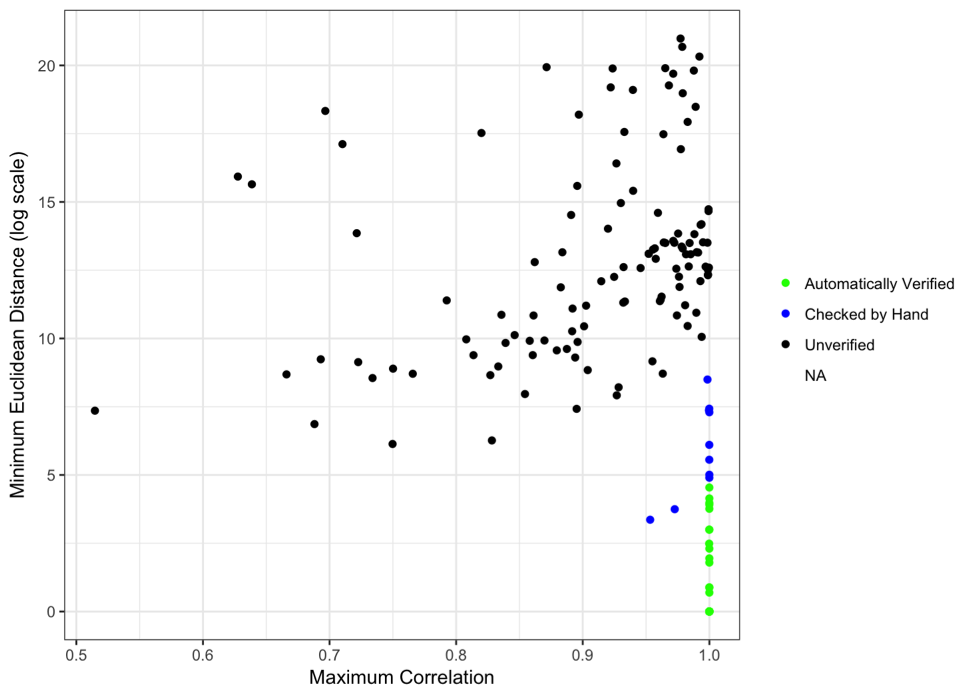
\includegraphics[width=0.70000\textwidth]{./figures/verification.png}
\caption{Classification of variables in raw 1890 census data after
comparing to the ICPSR 3 data.}
\end{figure}

Data were organized as follows. Each separate file corresponded to year.
Rows represented states, and columns corresponded to demographic
variables. Entries in the table were state-aggregated counts of number
of people in that category. Each state was given a label \texttt{Type}
as either a State or Territory, as some U.S. territories participated in
the decennial census before they received full statehood. Each
individual file is labeled as \texttt{states} followed by the year of
the census, (e.g. \texttt{states1790}) in this package. We combined the
state-level datasets into one list, \texttt{stateslist}, which is the
list of data that is used to populate the census browser.

\subsection{Description}

The package includes the state-aggregated data for each individual year,
as well as a list of all of the years together. We expect that users
will interact with these data sources via the Shiny application,
\texttt{Get\ Your\ Data}. This interactive Shiny application presents
the user with two options - focusing on a single year of the census,
found in the \texttt{Single\ Year} tab, or focusing on multiple years at
once, found in the \texttt{Multiple\ Years} tab.

The \texttt{Single\ Year} tab allows users to choose a year from a
drop-down menu; two manual-search entry boxes permit searching for
variables of interest. For example, if a user is interested in the
prevalence of farms in 1860, they can select 1860 and then search for
``farms'' in the first ``Variable of Interest'' field (see Figure 3).
Users will then see a complete list of all variable names in that
particular year that contain ``farms'' in their title. With this list
now available, users can select each variable they want by clicking on
it. Once all desired variables have been selected, clicking on the
``Download Filtered Data'' button will open a window in which the user
can choose a file name and directory location for saving the resulting
comma-separated values file. Variables will not remain selected if the
user chooses to change their search term or add a second search term.
However, if the user has interest in many separate variables that
require different search terms, it is easy to combine multiple csv files
in R using \texttt{full\_join} from the \texttt{dplyr} package and
specifying \texttt{State}, \texttt{Year}, \texttt{TOTAL.POPULATION}, and
\texttt{Type} as the variables by which to join. These four variables
will always be included in the resulting csv file, whether the user
selects them or not.

\begin{figure}[htbp]
\centering
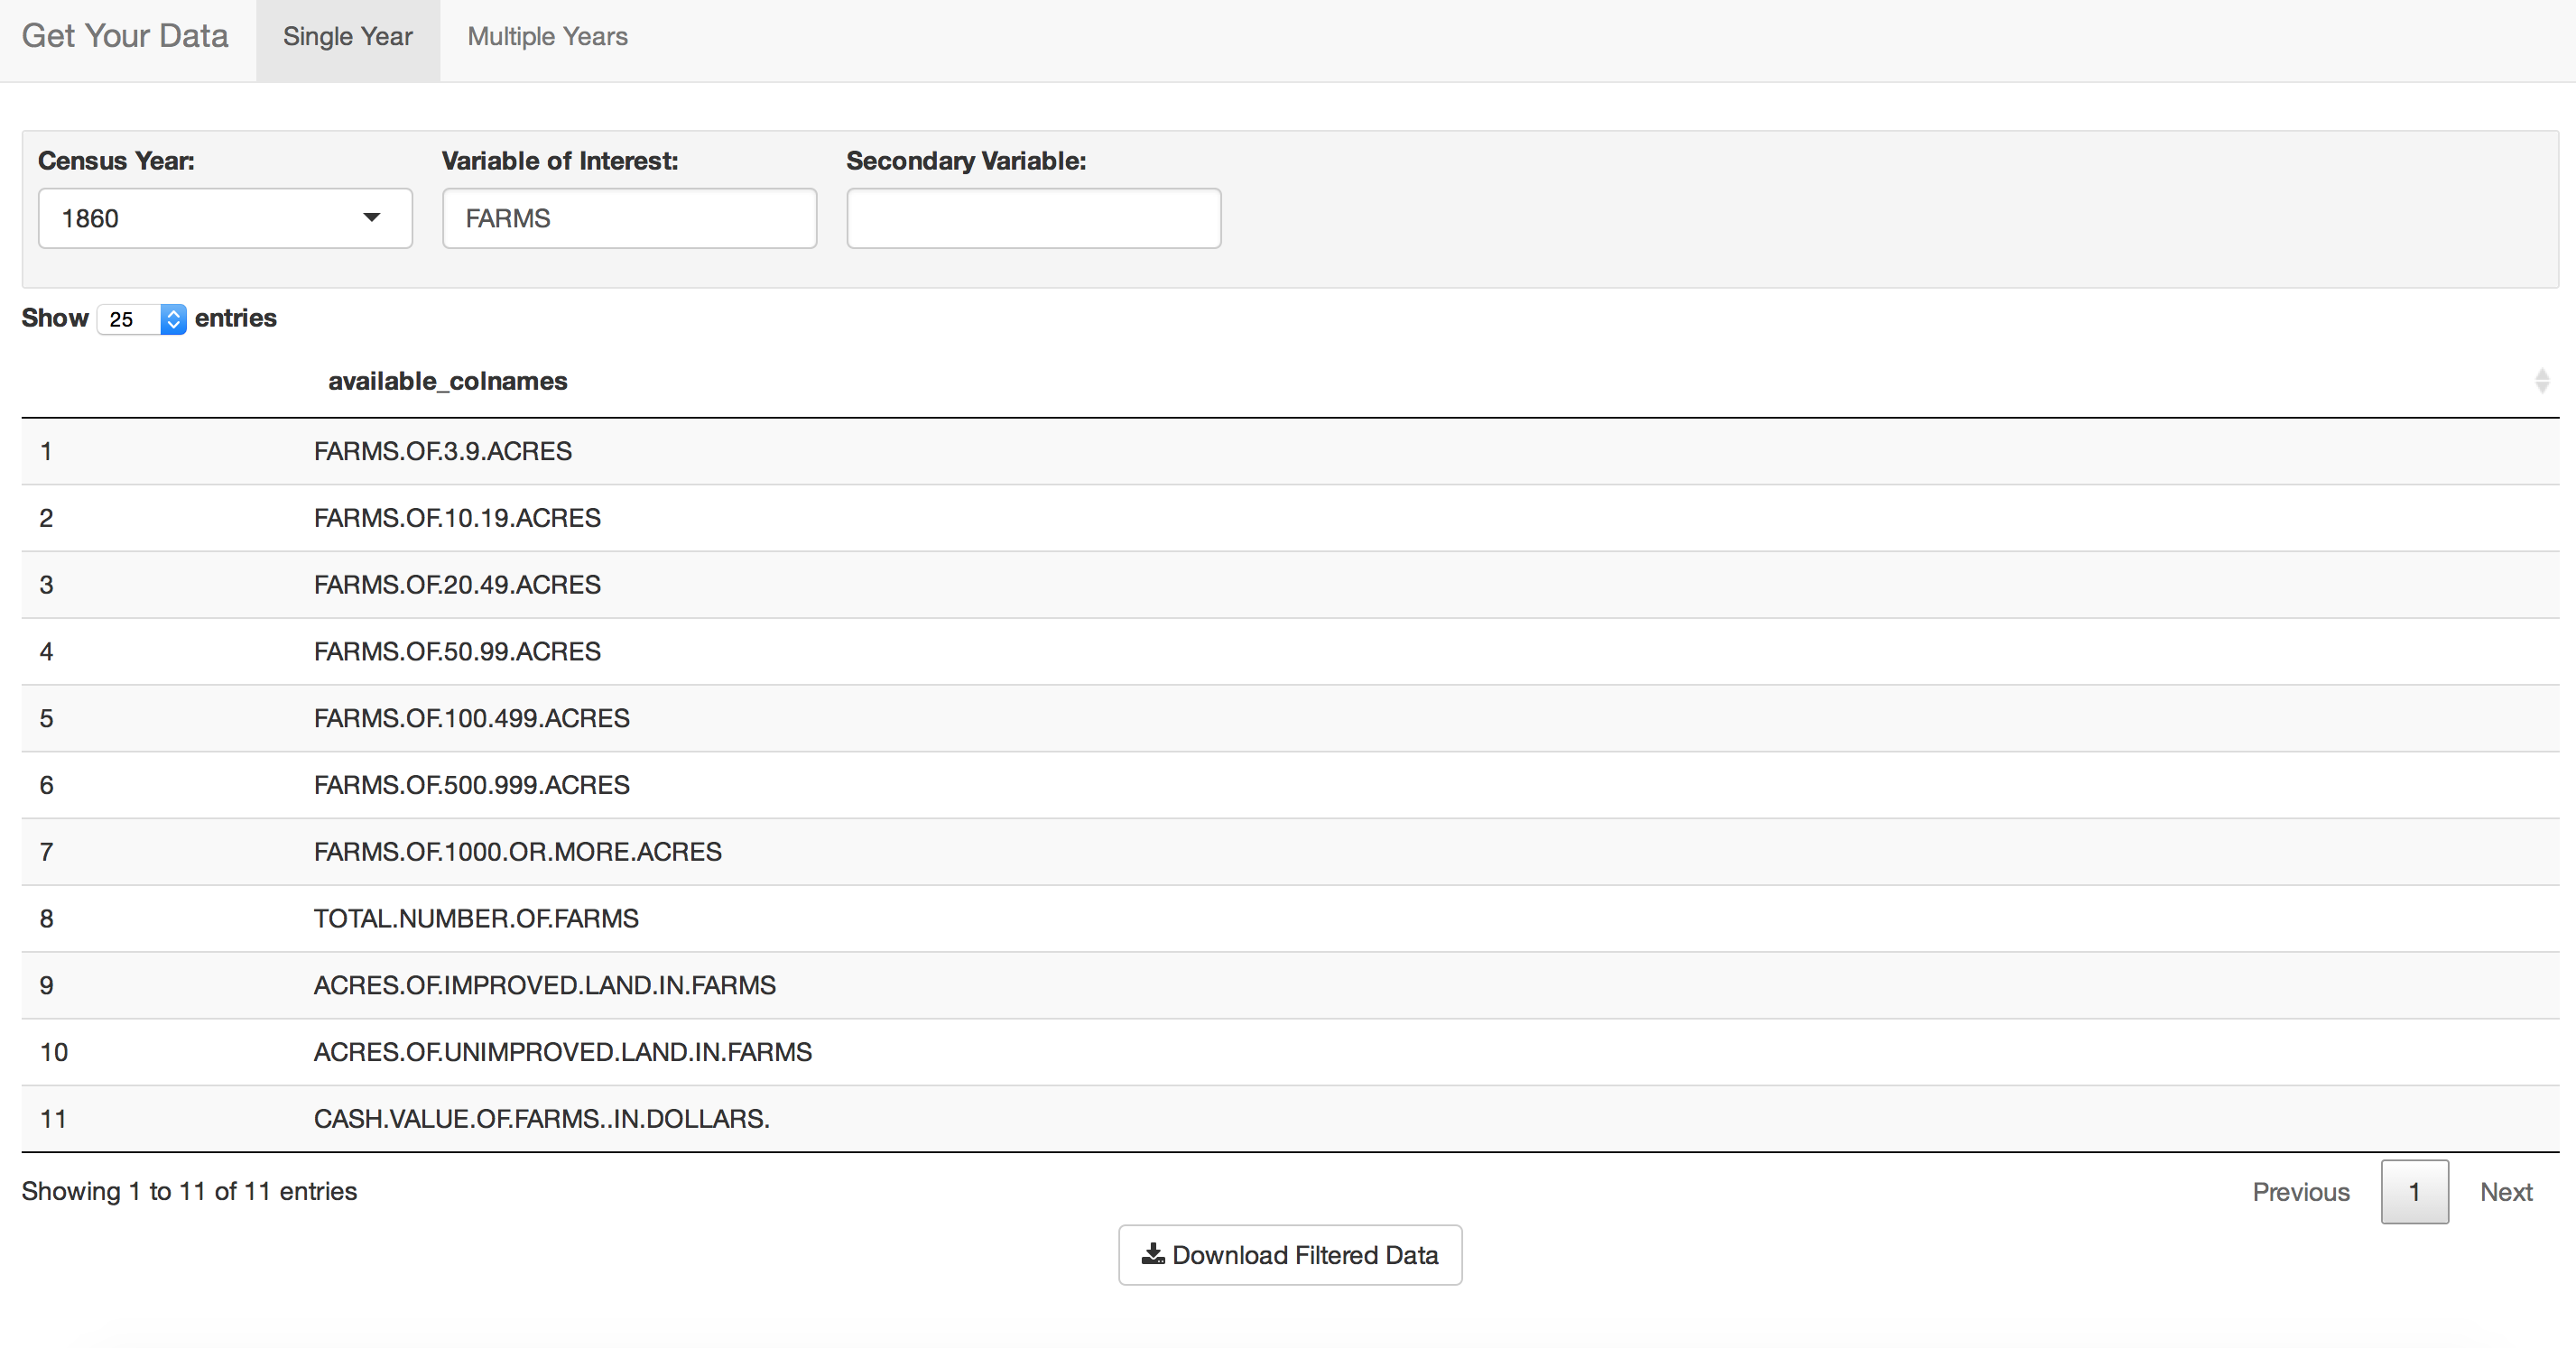
\includegraphics{./figures/app-sshot-farms.png}
\caption{The resulting view of a search for farms in the 1860 U.S.
Census on the \texttt{Single\ Year} tab of the \texttt{Get\ Your\ Data}
app.}
\end{figure}

The \texttt{Multiple\ Years} tab allows users to look for variables of
interest over a range of years. It offers all decennial censuses from
1790 to 1960, and includes the same search tool as before, but only
allows users to narrow down results by one search term rather than the
two provided in the \texttt{Single\ Year} tab. Users can select the
range of years in which they are interested by using the slider tool to
specify the range of interest, and subsequently use the ``Variable of
Interest'' search bar to narrow down their results. The results, which
are now two-dimensional rather than just a single list of available
variables, are presented somewhat differently in the
\texttt{Multiple\ Years} tab. Each available variable is listed along
the left side of the interface, and each selected year is presented
across the top as a column in the table (see Figure 4). For each
variable in the table, an \texttt{X} indicates whether the variable is
available in that particular year. Far to the right, there is a column
which indicates the number of selected years that include that
particular variable. Users can choose to order the results by this
count, if they wish. This is where it is important to remember that
variable names for different demographic groups can change drastically
over the course of the decennial census, and thus users will want to be
cognizant of varying search terms that may need to be checked. For some
of these terms, a notification will pop up for the user in the corner of
the app. The notification states that the term the user is searching for
may change over time. While this feature is not yet active for every
difference in the data, it can act as an early warning system for some
differences that we have already identified.

Similar to the output file of the \texttt{Single\ Year} tab, once a user
selects all variables of interest, she/he can select the ``Download
Filtered Data'' button to download a csv file of the chosen variables
for all states across the selected years. For years in the selected
range that do not include a particular variable, the csv file will be
filled in with \texttt{NA} values. This allows the structure of the data
table to remain intact although there are some year-variable
combinations that do not exist in the data. As mentioned previously,
because of the changing nature of variable names in the decennial
census, users may have to search for several separate terms, download
each file separately, and combine them once the files are downloaded.
The files can be combined using \texttt{full\_join} as we discussed
earlier. Multiple files are easy to combine because the structure
ensures that key variables needed to add on new columns are in place,
regardless of which variables users choose to download. This results in
one data table where each row represents a year-state combination and
all variables of interest are represented as columns. Users can easily
filter on specific variables or years while still maintaining the
original full data set, which is advantageous for visualizing how a
demographic group changes over time.

\subsection{Example}

The \texttt{Get\ Your\ Data} Shiny app can be used to search for a
topic, find the data of interest, download state-level information, and
tell a visual story of populations in the United States over time. To
demonstrate the utility of this Shiny app, we walk through an example on
the history of the African American population in the United States. We
begin by running the Shiny app:

\begin{Shaded}
\begin{Highlighting}[]
\KeywordTok{library}\NormalTok{(shiny)}
\NormalTok{shiny::}\KeywordTok{runGitHub}\NormalTok{(}\StringTok{"kiegan/censusbrowseR"}\NormalTok{, }\DataTypeTok{subdir =} \StringTok{"shiny"}\NormalTok{)}
\end{Highlighting}
\end{Shaded}

The default set of years is 1790 to 1880. However, the slider range can
be expanded to be able to explore data across all the available years.

\begin{figure}[htbp]
\centering
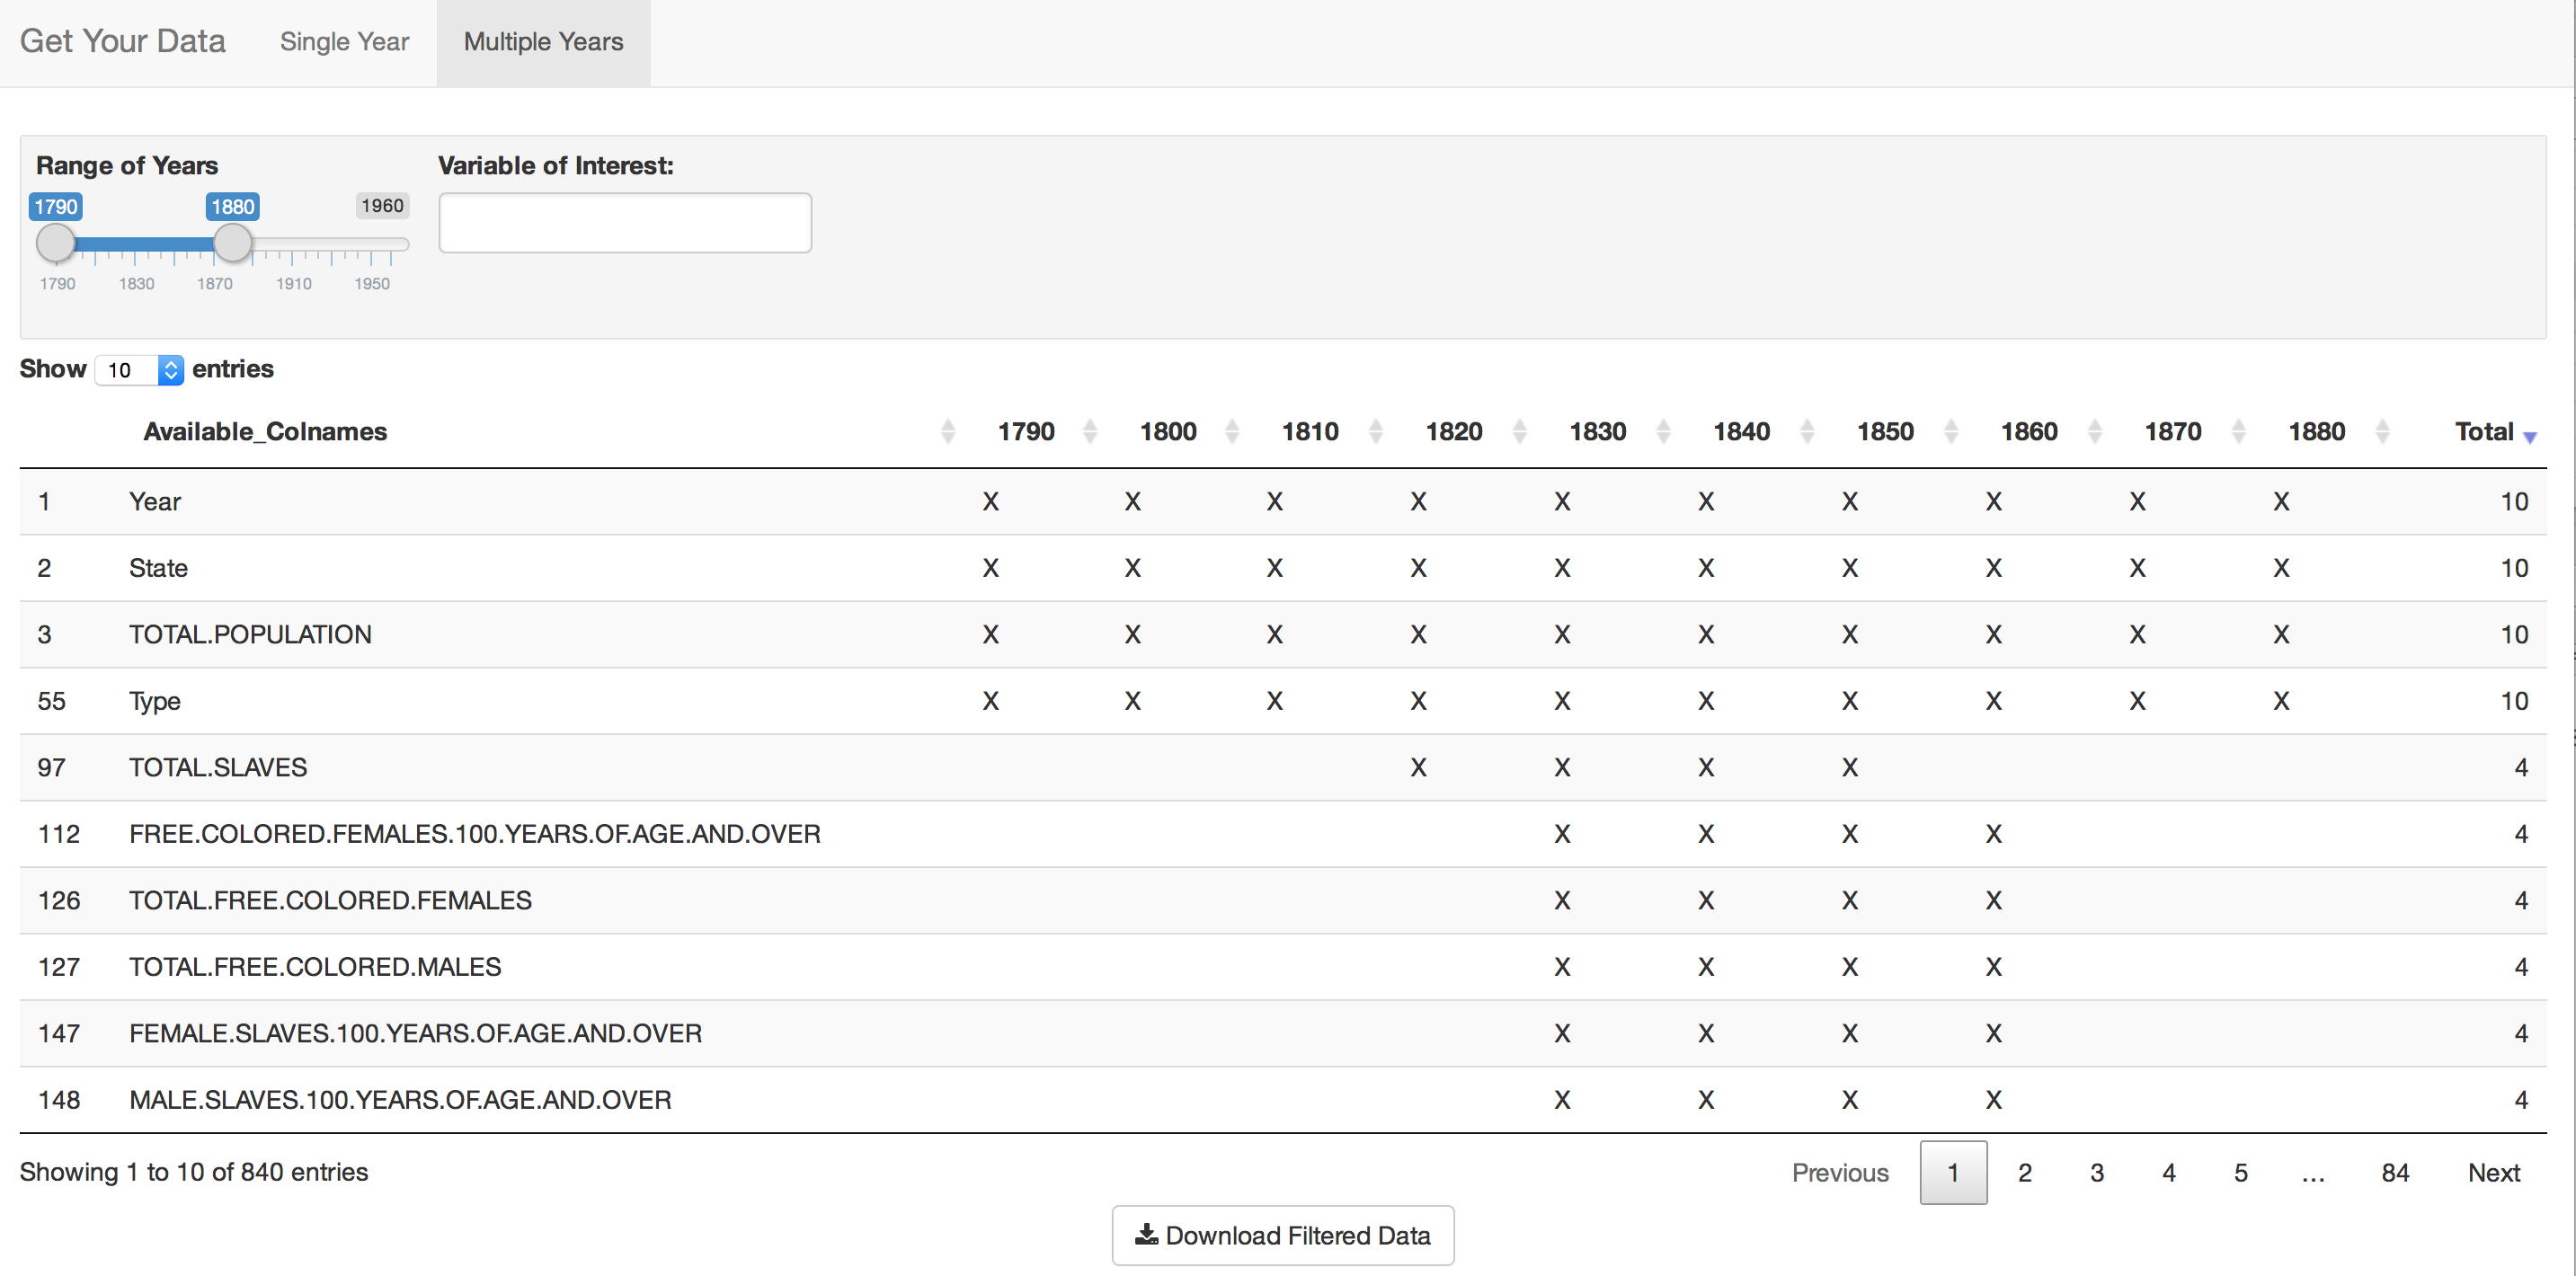
\includegraphics{./figures/app-sshot-multiple-years.png}
\caption{An example of available column names for the years 1790 to
1880.}
\end{figure}

After ordering by how many years each variable appears in, the available
variable names show a serious lack of continuity. The four ever-present
variables (\texttt{Year}, \texttt{State}, \texttt{TOTAL.POPULATION}, and
\texttt{Type}) each appear ten times, once in each year selected. After
that, the next most common variable only appears in four of the ten
years we have chosen. This highlights some of the hurdles that we will
encounter when tracking any demographic group over time.

Since the focus will be on African Americans throughout U.S. history,
the first search term needed is \texttt{SLAVE} in the early years of the
U.S. census. The vast majority of African Americans were slaves when the
United States was founded, so variables that count the number of slaves
tell the story about the African American population in early U.S.
history. Note that the \texttt{SLAVE} categorization is the only term
the U.S. census had related to African Americans in the early years of
the census, so it is also the only source of information available on
that group for that time period.

Once we have selected a range of years, we then enter a search term.
Searching for \texttt{SLAVE} results in a list of all the candidate
variable names across all years, which can again be sorted by their
frequency across years. The results of this search can be seen in Figure
5.

\begin{figure}[htbp]
\centering
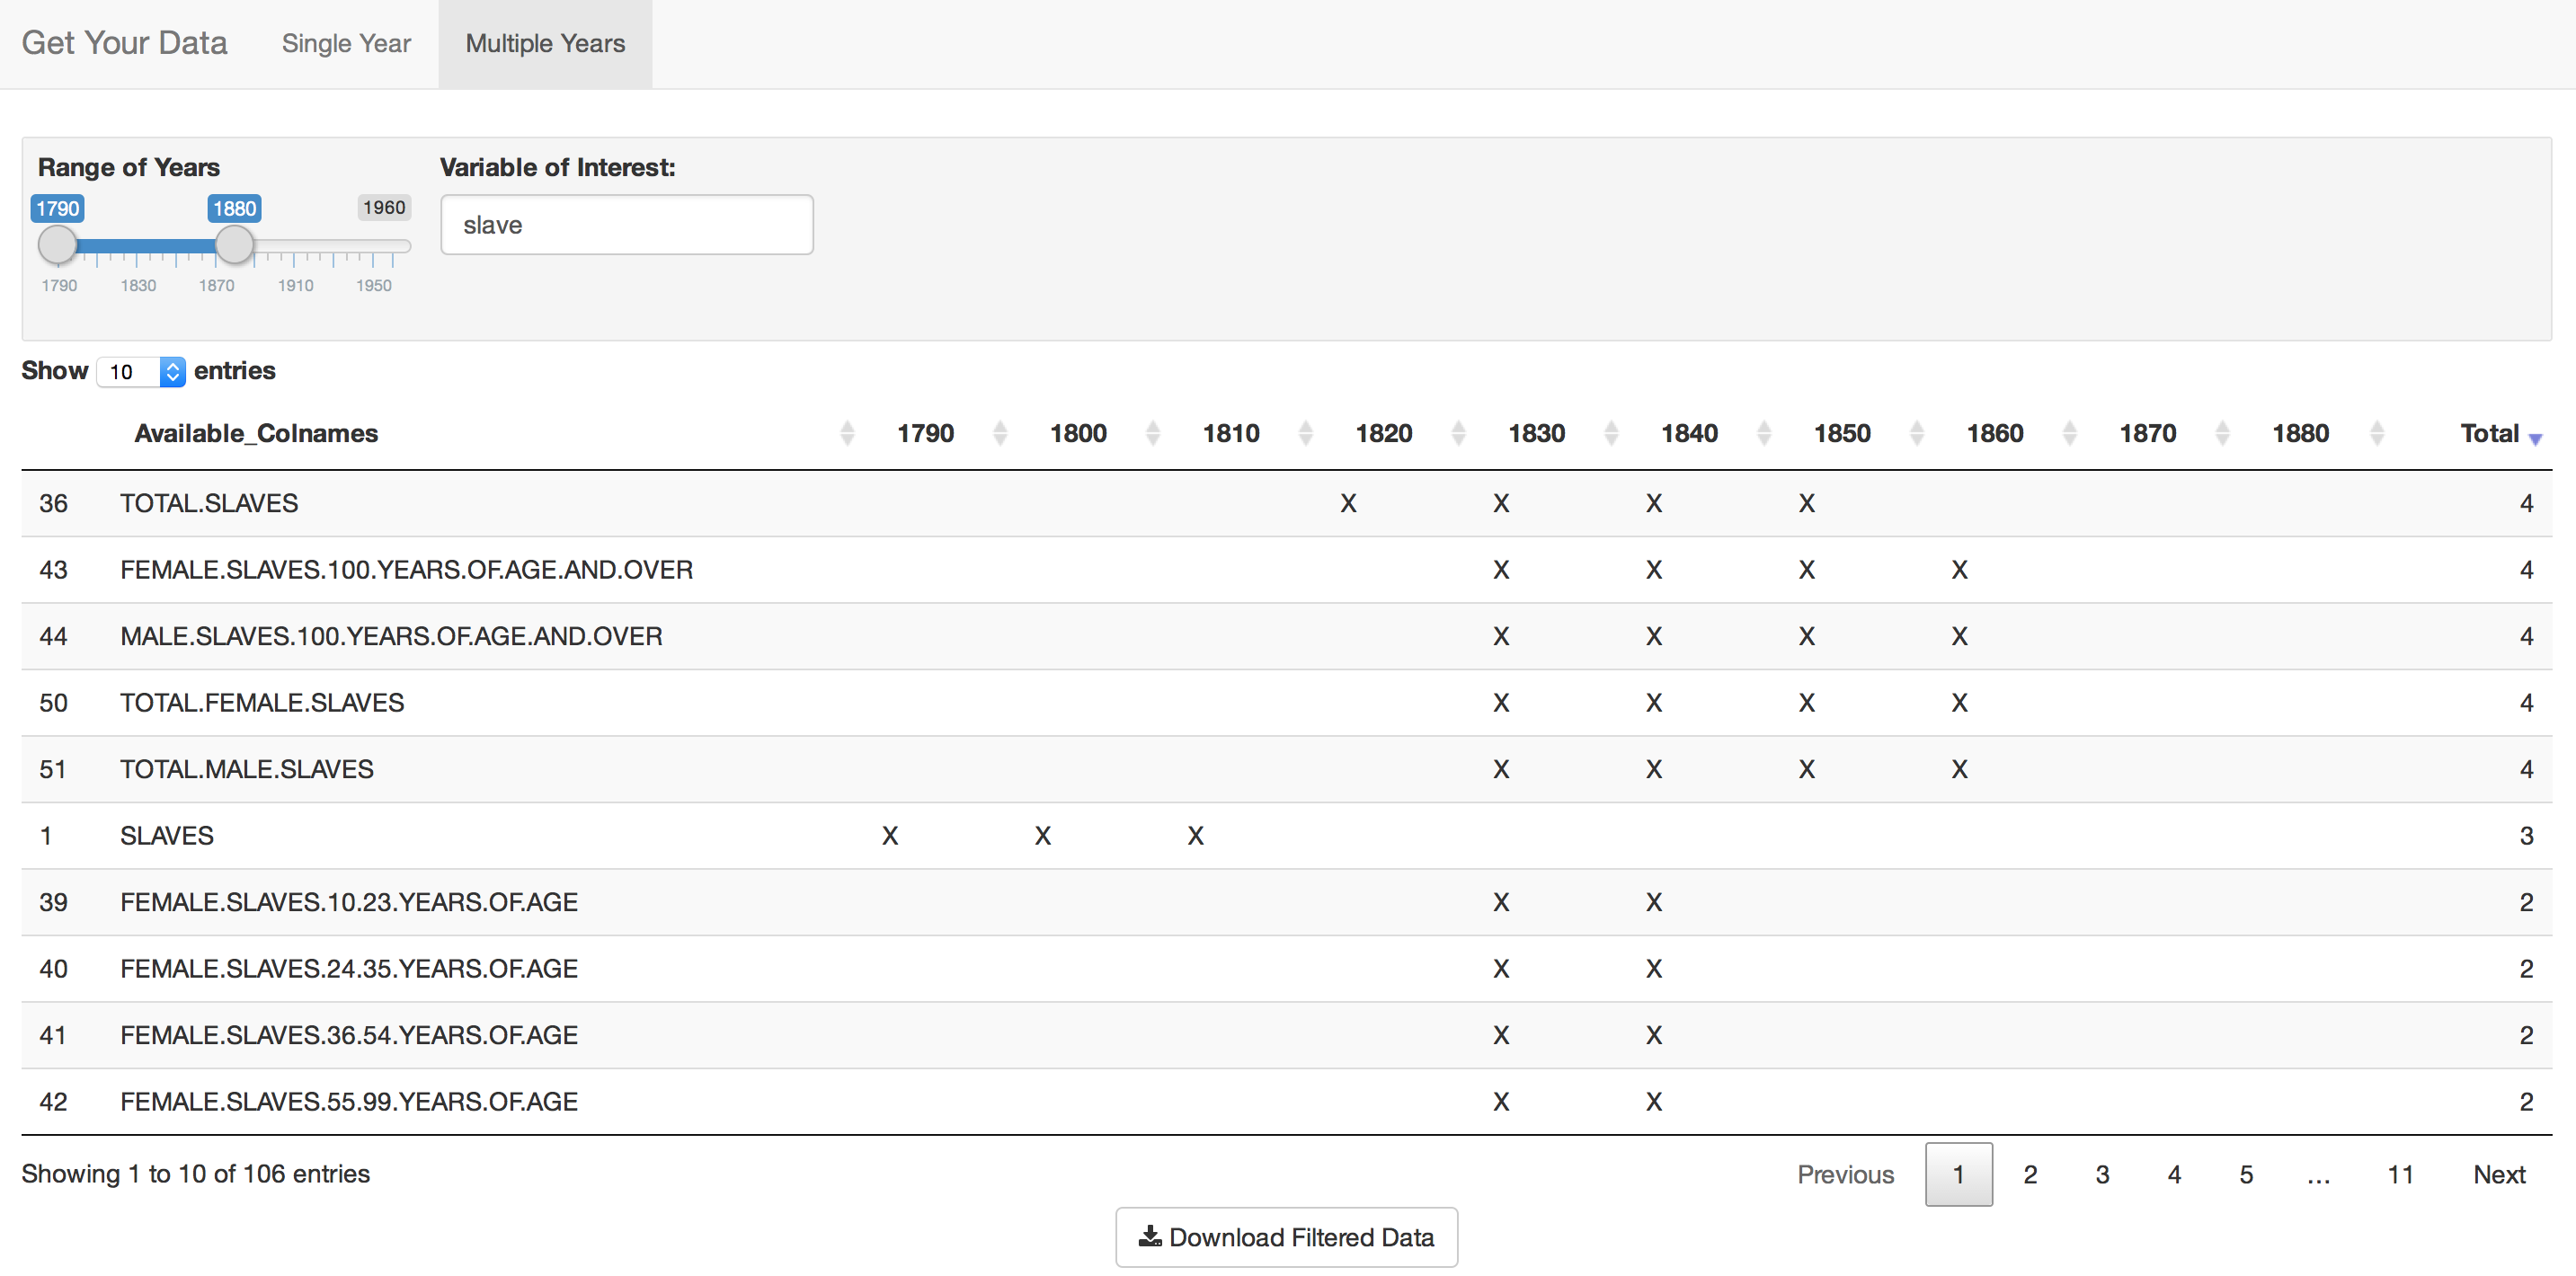
\includegraphics{./figures/app-sshot-slave.png}
\caption{The resulting table after searching for the term `slave' in the
\texttt{Get\ Your\ Data} app.}
\end{figure}

For this example, we executed three separate searches within the
\texttt{Get\ Your\ Data} app, using three different terms that the
census used to categorize African Americans at different points in the
decennial census (``slave'', ``colored'', and ``negro''). The third of
these terms, when used for plotting, will be labeled as ``black'' for
the remainder of the example. This gave three separate csv files, which
were combined using the function \texttt{full\_join} from the
\texttt{dplyr} package. Now, for this demographic group, all of the
state-aggregated population counts are together in one data frame,
although different terms are used at different points in time.

The combined data can now be explored. For any particular year, a subset
of the full dataset can be taken to include only information for that
year. This allows for quicker determination of which variables are
available for that particular year. For example, after subsetting on the
year 1790, state-level counts of the \texttt{SLAVES} variable for that
year can be plotted. Use of the \texttt{USAboundaries} package in
concert with this census browser is recommended, as it provides the most
accurate boundaries of the United States at any given date (Mullen and
Bratt 2017). Just as variable names and the make-up of the census
rapidly changed throughout the United States' history, the boundaries of
the states and territories changed as well. The recorded
state-aggregated values in the dataset are for the states as they
existed during that census year, and thus sometimes include demographic
counts from areas that differ from the currently defined state
boundaries.

\begin{figure}[htbp]
\centering
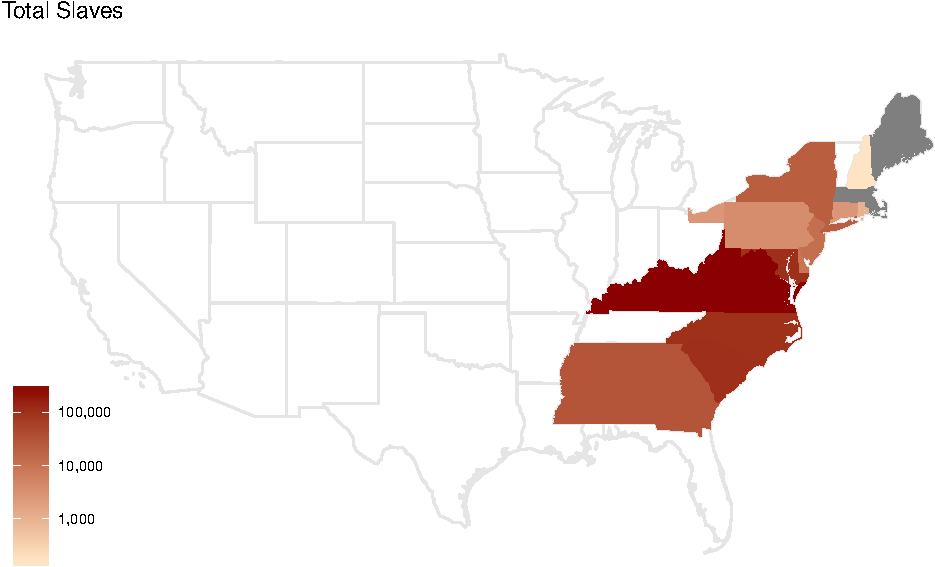
\includegraphics{writeup_files/figure-latex/chunk-1790-map-1.pdf}
\caption{Total number of slaves per state in 1790, plotted on a
continuous log scale. State boundaries for July 4, 1790 were gathered
from \texttt{USAboundaries} package.}
\end{figure}

With a visualization of the slave population in the United States in
1790 in hand (see Figure 6), it is possible to look at subsequent years
of the decennial census in a similar manner to see how the population
changes over time.

\begin{figure}[htbp]
\centering
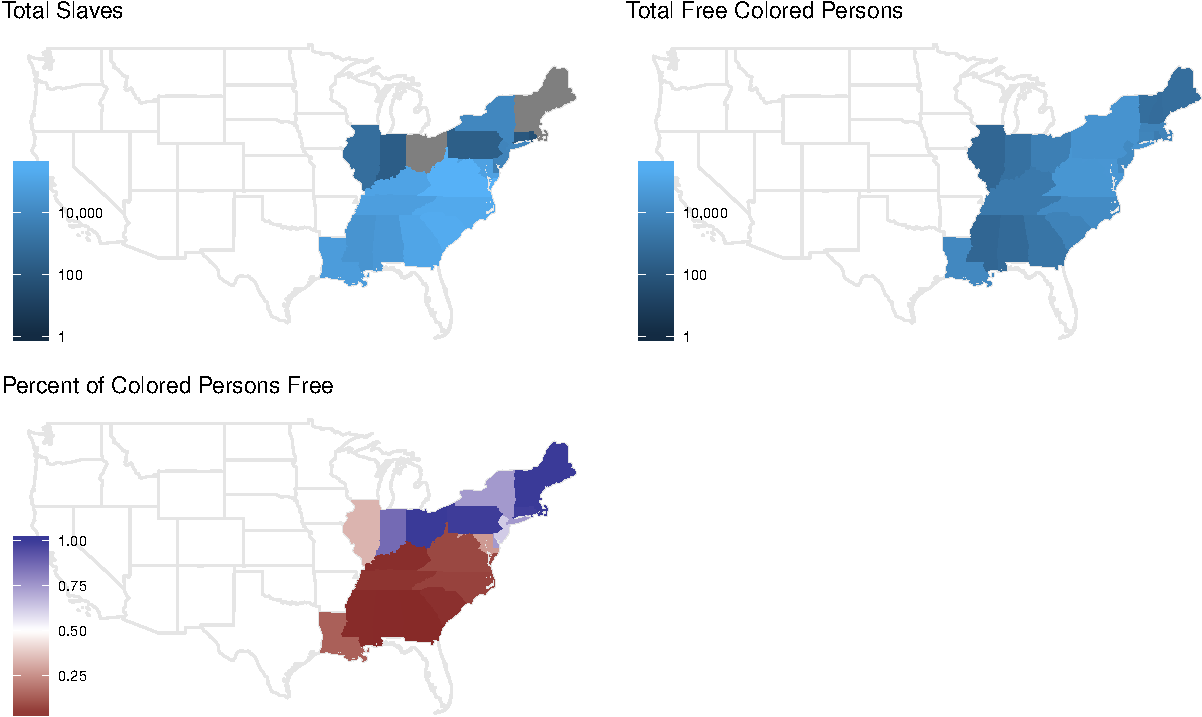
\includegraphics{writeup_files/figure-latex/unnamed-chunk-5-1.pdf}
\caption{Number of Slaves, Number of Free Colored Persons, and
Percentage of Free Colored Persons in 1820.}
\end{figure}

Jumping to the year 1820, and again filtering on that particular year,
we learn new information about the African American population. The
census at this time includes a count of
\texttt{TOTAL.FREE.COLORED.PERSONS}, as there are citizens who are
African American or other minorities that are free, and not slaves. At
this time, many minorities were grouped together in the ``colored
persons'' category, and as before, we do not have any other record for
African Americans except this categorization and the ``slaves''
categorization. However, since the 1820 census included records for both
\texttt{TOTAL.FREE.COLORED.PERSONS} and \texttt{TOTAL.SLAVES}, we can
also now visualize the percentage of African Americans in each state
that were categorized as ``free persons'' as opposed to slaves (see
Figure 7). Knowing that both of these variables are available allows for
a powerful comparison by visualizing the growing divide between northern
and southern states in the United States at that time.

\begin{figure}[htbp]
\centering
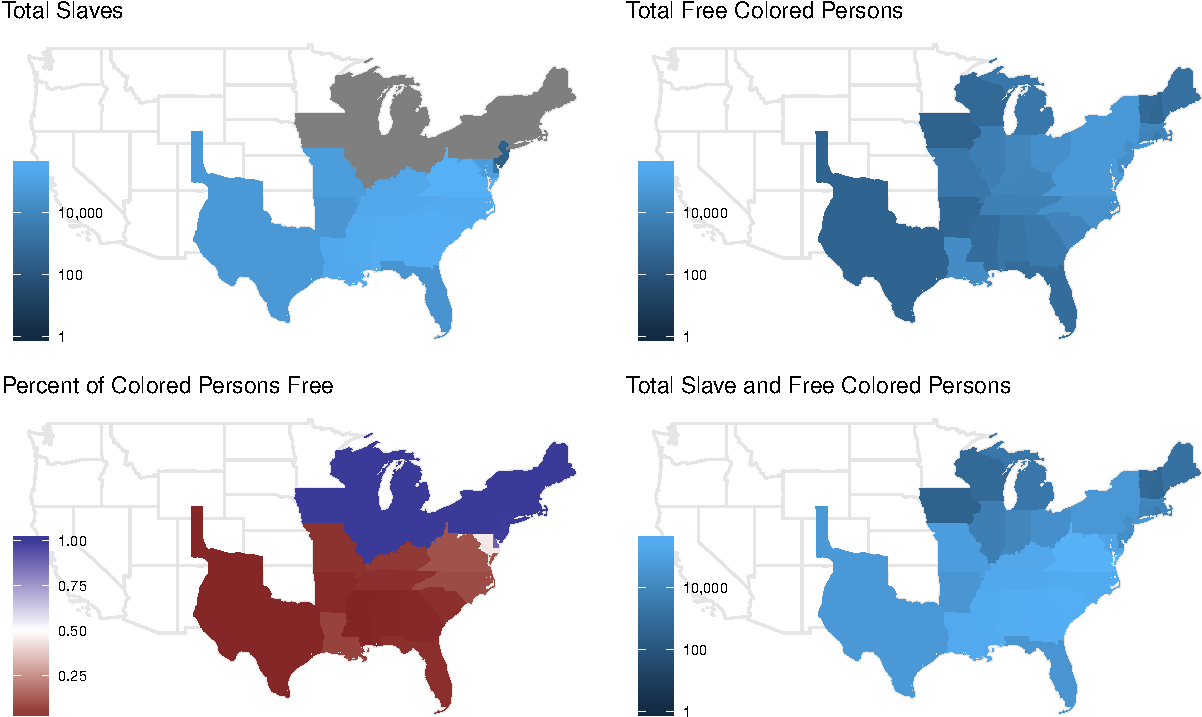
\includegraphics{writeup_files/figure-latex/unnamed-chunk-6-1.pdf}
\caption{Number of Slaves, Number of Free Colored Persons, Percentage of
Free Colored Persons, and Total Colored Persons in 1850.}
\end{figure}

Moving forward in time, even more information can be gleaned about this
population. When we subset on the year 1850, we see that although there
is still a \texttt{TOTAL.SLAVES} column in the record, many states no
longer record this variable; by then, they had already abolished
slavery. We can transform these \texttt{NA} values into zeros to account
for this difference in the data and allow us to still calculate the
percentages of free African Americans. Starting in 1850, we can also
start investigating what the total African American population looks
like in each state, beyond just the size of the slave population and
freed population (see Figure 8).

\begin{figure}[htbp]
\centering
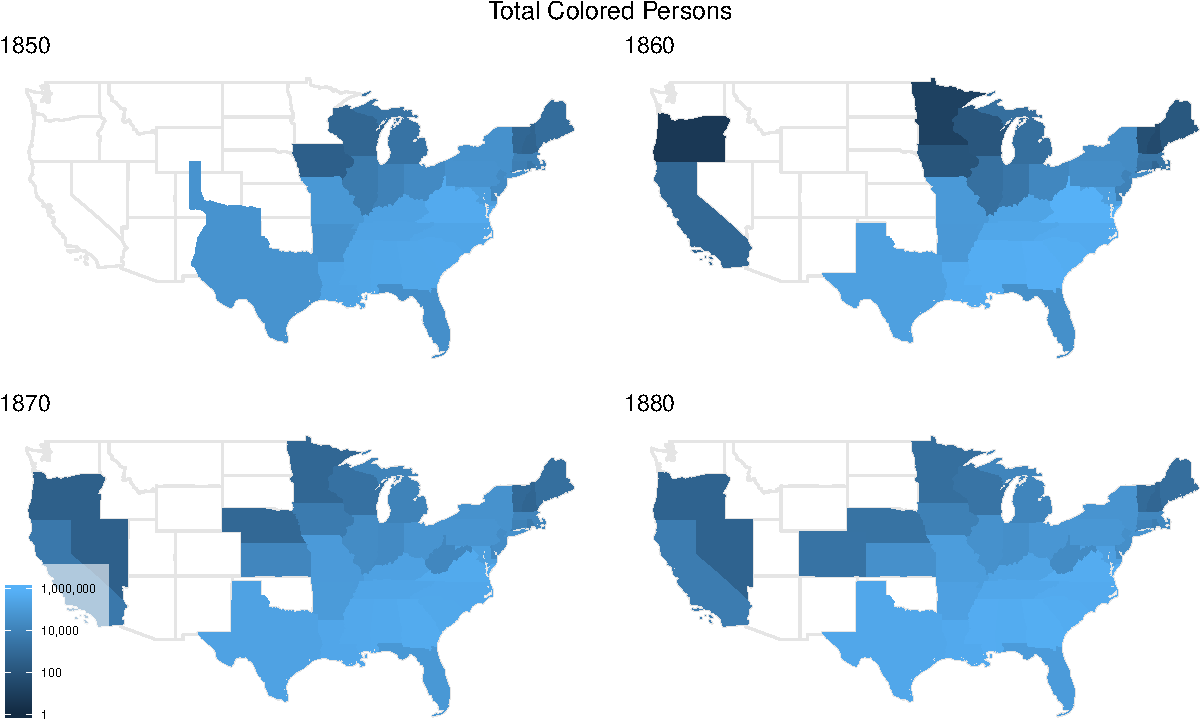
\includegraphics{writeup_files/figure-latex/unnamed-chunk-7-1.pdf}
\caption{Total Colored Persons in 19th Century United States}
\end{figure}

The total African American population is particularly interesting moving
forward after slavery is abolished in the 1860s and some migration
begins to occur out of certain areas. The balance of the total African
American population in each state begins to change as the United States
transitions into the post-slavery period (see Figure 9). We also see how
the boundaries of states change and new states are formed, with the
United States gaining new states at each census.

\begin{figure}[htbp]
\centering
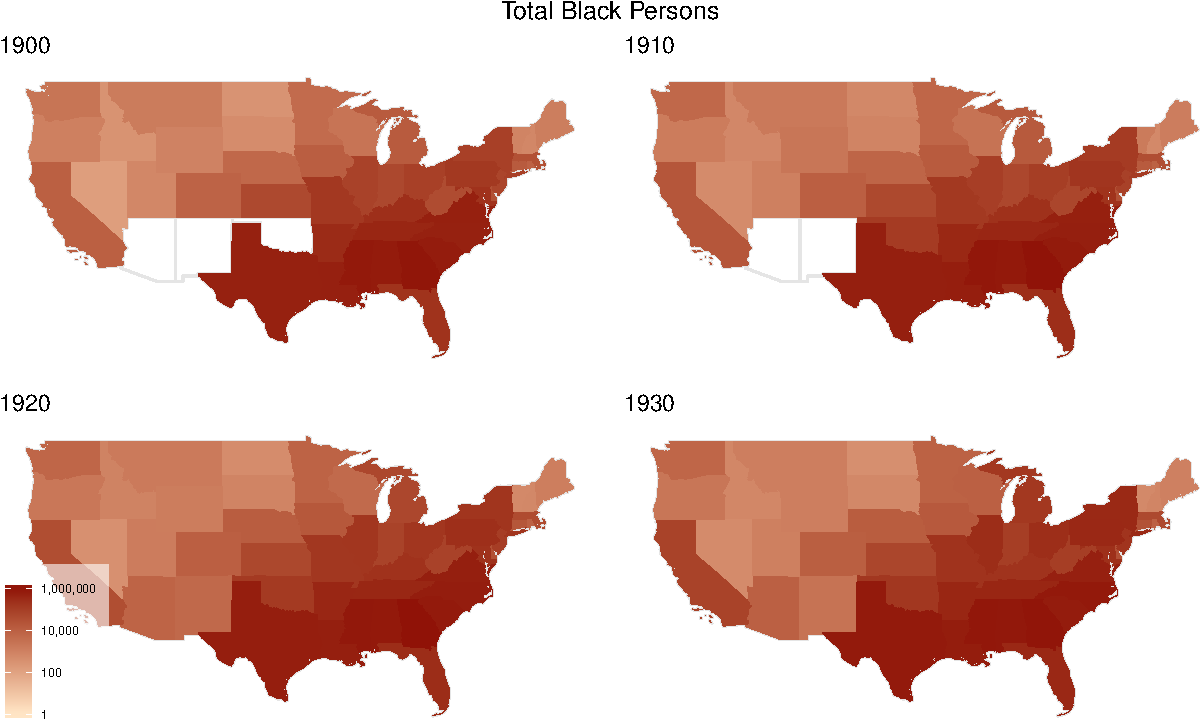
\includegraphics{writeup_files/figure-latex/unnamed-chunk-8-1.pdf}
\caption{Total Black Persons in 20th Century United States}
\end{figure}

A period of growth and change can be seen at the turn of the 20th
century as well, with a dramatic shift in the African American
population out west to California and with the balance in the east and
midwest shifting slightly further north (see Figure 10). Although the
highest density of colored persons is still in the southern states, we
can see that of a northern migration is taking place.

\section{Discussion}

The decennial census is a rich source of historical information. We have
built a tool that can help extract and visualize that information to,
for example, understand how demographic attributes of the U.S.
population have changed over time.

Although there is no county-level information available and the data for
the census browser go only through 1960, users are able to efficiently
explore variables of interest at different time points in U.S. history
and tell a visual story about a growing nation and a changing
population. This connectivity across years and ability to assess what
information was available when, all in one browser, have the potential
to save time and effort of researchers interested in delving into United
States history.

The structure of our browsers also helps determine not only the
variables that are available in a given year, but also where information
is missing for some states on a particular variable. Finding these
differences is easier when all relevant varialbes are combined in one
data frame, which can be summarized and searched all at one time.

\section{Ongoing Work}

To investigate even more complex patterns in United States history, it
would be helpful to have a finer grid of information - specifically
county-level data. There are inherent challenges with a more complex set
of data such as county-level, such as lack of continuity across counties
and states. Another big challenge would be to construct a layout in
which users can interact with years, but also with differences across
locales to find the most complete information about variables of
interest. Despite these anticipated challenges, adding county-level data
to this browser would give researchers a much richer resource with which
to work.

The census adapts and changes with each passing decade. Different
variables are tracked, congressional boundaries change, and the
demographic landscape of the United States changes as well. If we could
add current information (through 2010) and if we were able to update
information as it is collected we would then be able to juxtapose
today's population with that of the past. Being able to put history into
context is important, and an up-to-date census browser could help
students and researchers alike who wish to work with historical census
information.

\section{References}

\hypertarget{refs}{}
\hypertarget{ref-Shiny}{}
Chang, W., J. Cheng, JJ. Allaire, Y. Xie, and J. McPherson. 2017.
``Shiny: Web Application Framework for R.'' Computer Program.
\url{http://CRAN.R-project.org/package=shiny}.

\hypertarget{ref-ChartInterview}{}
Hofmann, Heike. 2007. ``Interview with a Centennial Chart.'' Journal
Article. \emph{CHANCE} 20:2: 26--35.

\hypertarget{ref-USAboundaries}{}
Mullen, L., and J. Bratt. 2017. ``USAboundaries: Historical and
Contemporary Boundaries of the United States of America.'' Computer
Program. \url{http://cran.r-project.org/web/packages/USAboundaries}.

\hypertarget{ref-StatisticalAtlas}{}
Office, United States Census, and F. A. Walker. 1874. \emph{Statistical
Atlas of the United States Based on the Results of the Ninth Census 1870
with Contributions from Many Eminent Men of Science and Several
Departments of the Government}. Map.
\url{https://www.loc.gov/item/05019329/}.

\hypertarget{ref-RCoreTeam}{}
R Core Team. 2015. ``R: A Language and Environment for Statistical
Computing.'' Journal Article. \url{http://www.R-project.org}.

\hypertarget{ref-HCB}{}
Virginia Library, University of. 2017. ``Historical Census Browser.''
\url{https://mapserver.lib.virginia.edu/}.


\end{document}
